\documentclass[report.tex]{subfiles}
\begin{document}
\subsection{Methodology}
The RF filters discussed in this report can be divided in 3 sections
\begin{itemize}
    \item Lumped 2\nd order maximally flat band-pass filter
    \item Distributed 2\nd order flat band-pass filter on RO4350B substrate
    \item Distributed 2\nd order flat band-pass filter on FR-4 substrate
\end{itemize}
For each filter design, the attenuation at pass- and stop-band limits (table \ref{table:filter specs}) was measured. A summary of measured attenuation is found in table \ref{table:attenuation summary}.

All filters were designed using ADS DesignGuide (\emph{Filter/Filter Control Window} or \emph{Passive Circuit/Microstrip Control Window}).

Two different types of simulations was performed on the distributed filters: schematic and layout simulation. The Schematic simulation can be launched directly from the DesignGuide control window. To do a layout simulation, a layout has to be either created or generated.

The layout was generated by first designing the filter with DesignGuide, \emph{push into hierarchy} of the filter and then select \emph{Layout/(Generate/Update layout)}. The substrate of the layout was then imported from the main schematic.

The layout simulation can then be launched from the menu of the layout design window. All layout simulations of this report are performed with a [1.0,3.0] GHz frequency span.

\subsubsection{Lumped 2\nd order maximally flat band-pass filter}
From the DesignGuide \emph{Filter/Filter Control Window}, a double terminated bandpass filter was chosen (see fig.~\ref{fig:Filter A}) and the specifications from table \ref{table:filter specs} was filled in. The filter order was also entered. 

The simulation frequency span was automatically determined by DesignGuide to [1.94,2.94] GHz.

\begin{figure}[h]
    \centering
    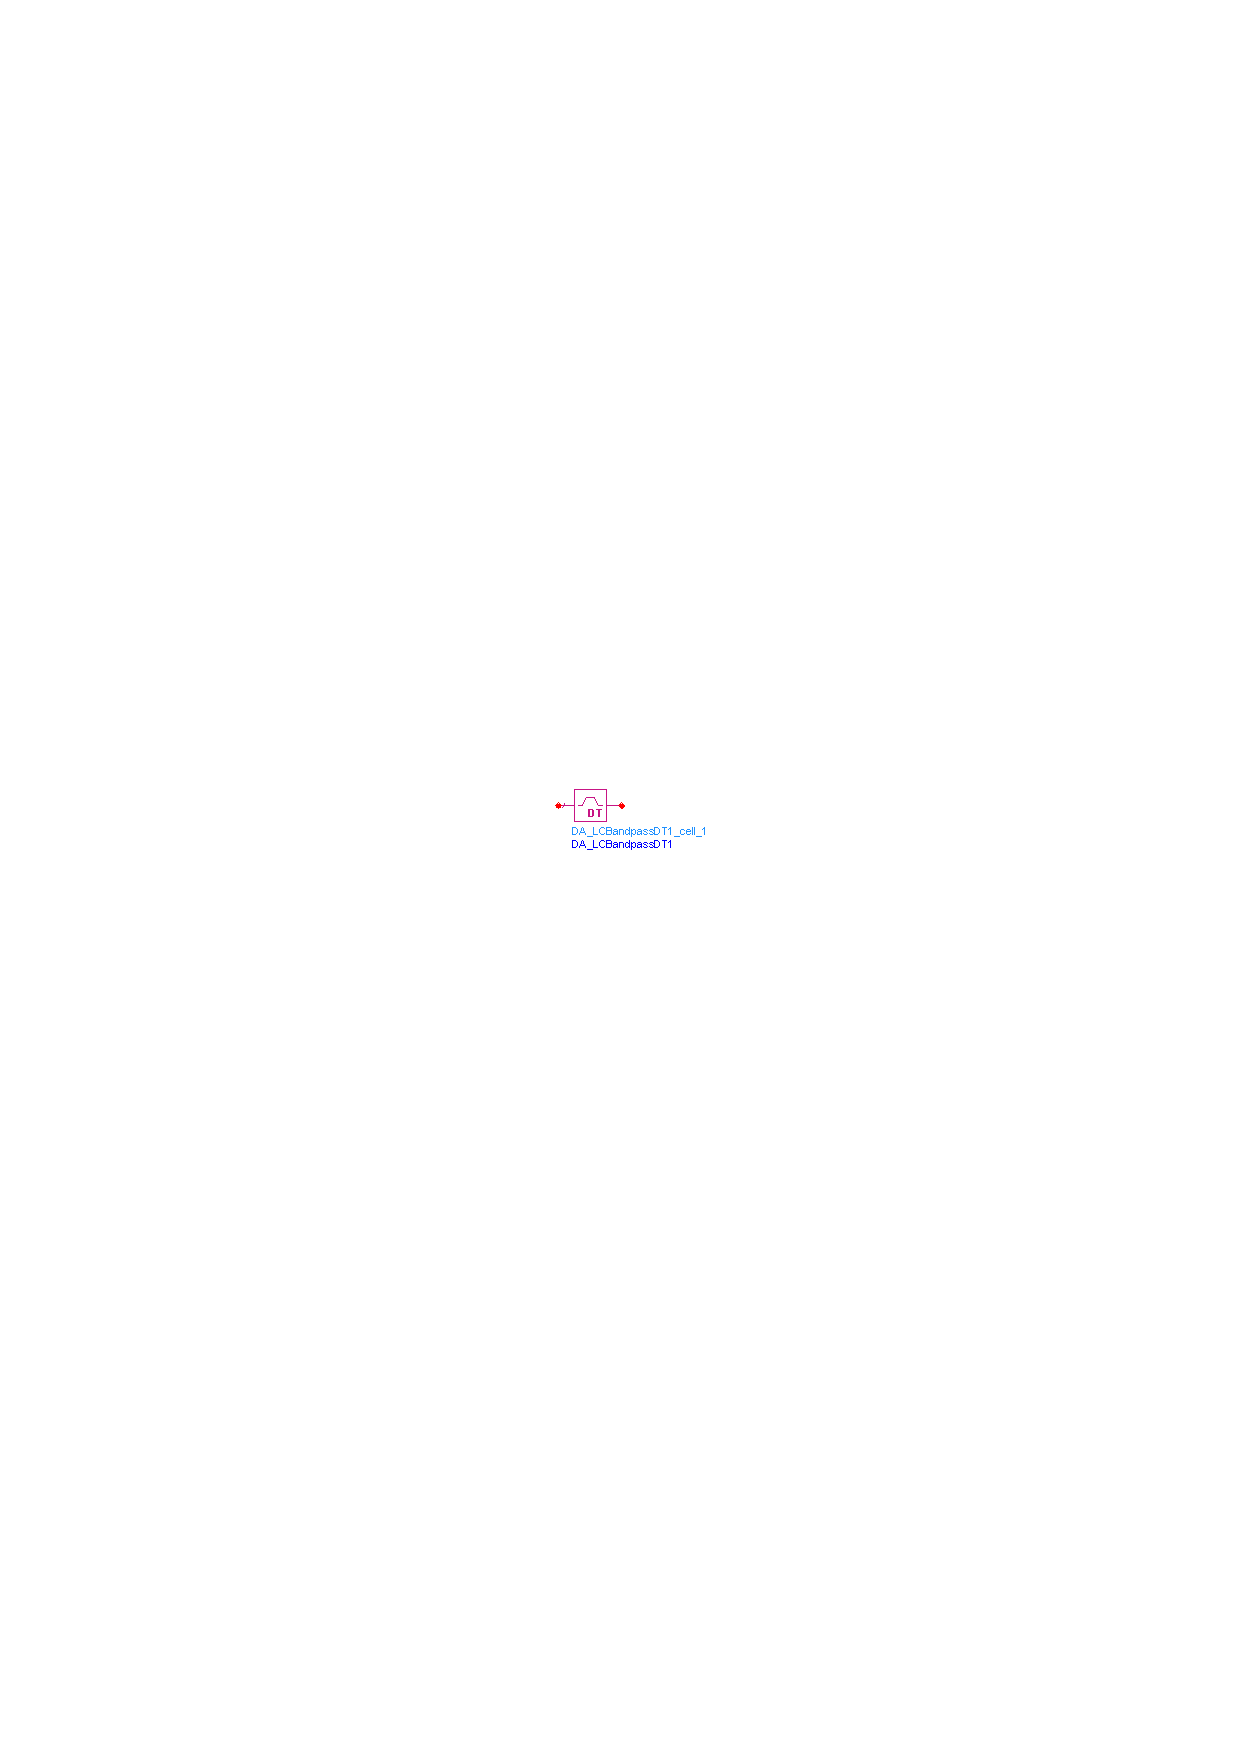
\includegraphics[scale=2]{design_guide_symbol}
    \caption{Double terminated bandpass filter schematic symbol}
    \label{fig:Filter A}
\end{figure}

\subsubsection{Distributed 2\nd order maximally flat band-pass filter (RO4350B)}


\subsubsection{Distributed 2\nd order maximally flat band-pass filter (FR-4)}

\end{document}